\documentclass[twoside,openright,titlepage,fleqn,
	headinclude,11pt,a4paper,BCOR5mm,footinclude
	]{scrbook}
%--------------------------------------------------------------
        \newcommand{\myTitle}{Analisi di reti metaboliche basata su
          propriet\`a di connessione\xspace}
% use the right myDegree option
\newcommand{\myDegree}{Corso di Laurea in Informatica\xspace}
%\newcommand{\myDegree}{
	%Corso di Laurea Specialistica in Scienze e Tecnologie 
	%dell'Informazione\xspace}
\newcommand{\myName}{Massimo Nocentini\xspace}
\newcommand{\myProf}{Pierluigi Crescenzi\xspace}
\newcommand{\myOtherProf}{Nome Cognome\xspace}
\newcommand{\mySupervisor}{Nome Cognome\xspace}
\newcommand{\myFaculty}{
	Facolt\`a di Scienze Matematiche, Fisiche e Naturali\xspace}
\newcommand{\myDepartment}{
	Dipartimento di Sistemi e Informatica\xspace}
\newcommand{\myUni}{\protect{
	Universit\`a degli Studi di Firenze}\xspace}
\newcommand{\myLocation}{Firenze\xspace}
\newcommand{\myTime}{Anno Accademico 2010-2011\xspace}
\newcommand{\myVersion}{Version 0.1\xspace}
%--------------------------------------------------------------
\usepackage[latin1]{inputenc} 
\usepackage[T1]{fontenc} 
\usepackage[square,numbers]{natbib} 
\usepackage[fleqn]{amsmath}  
\usepackage[italian]{babel}
%--------------------------------------------------------------
\usepackage{dia-classicthesis-ldpkg} 
%--------------------------------------------------------------
% Options for classicthesis.sty:
% tocaligned eulerchapternumbers drafting linedheaders 
% listsseparated subfig nochapters beramono eulermath parts 
% minionpro pdfspacing
\usepackage[eulerchapternumbers,subfig,beramono,eulermath,
	parts]{classicthesis}
%--------------------------------------------------------------
\newlength{\abcd} % for ab..z string length calculation
% how all the floats will be aligned
\newcommand{\myfloatalign}{\centering} 
\setlength{\extrarowheight}{3pt} % increase table row height
\captionsetup{format=hang,font=small}
%--------------------------------------------------------------
% Layout setting
%--------------------------------------------------------------
\usepackage{geometry}
\geometry{
	a4paper,
	ignoremp,
	bindingoffset = 1cm, 
	textwidth     = 13.5cm,
	textheight    = 21.5cm,
	lmargin       = 3.5cm, % left margin
	tmargin       = 4cm    % top margin 
}
%--------------------------------------------------------------
\usepackage{listings}
\usepackage{hyperref}
% My Theorem
\newtheorem{oss}{Observation}[section]
\newtheorem{exercise}{Exercise}[section]
\newtheorem{thm}{Theorem}[section]
\newtheorem{cor}[thm]{Corollary}

\newtheorem{lem}[thm]{Lemma}

\newcommand{\vect}[1]{\boldsymbol{#1}}

% questo comando e' relativo alle correzioni che puo
% apportare il prof se lo desidera.
\newcommand{\prof}[1]{\boldsymbol{#1}}

% instead of boldsymbol I can use the arrow above the letter with
%\newcommand{\vect}[1]{\vec{#1}}

% page settings
% \pagestyle{headings}
%--------------------------------------------------------------
\begin{document}
\frenchspacing
\raggedbottom
\pagenumbering{roman}
\pagestyle{plain}
%--------------------------------------------------------------
% Frontmatter
%--------------------------------------------------------------
\include{titlePage}
\pagestyle{scrheadings}
%--------------------------------------------------------------
% Mainmatter
%--------------------------------------------------------------
\pagenumbering{arabic}

% settings for the lstlisting environment
\lstset{
	language = java
	, numbers = left 
	, basicstyle=\sffamily%\footnotesize
	%, frame=single
	, tabsize=2
	, captionpos=b
	, breaklines=true
	, showspaces=false
	, showstringspaces=false
}

\tableofcontents

\newpage
% \input{licences.tex}

% \newpage
% \input{sinopsi.tex}

% \newpage
% 
\section{Syntax and Format}

Nel documento i termini \emph{vertice} e \emph{nodo} sono da
considerarsi equivalenti e per questo verranno utilizzati in modo
interscambiabile.




Il mio lavoro inizia con lo studio e l'utilizzo del formato
\textbf{SBML} (\textbf{S}ystems \textbf{B}iology \textbf{M}arkup 
\textbf{L}anguage). 

Questo formato permette di rappresentare informazioni seguendo uno
schema gerarchico, basato su XML. Questo formato \`e orientato alla
descrizione di sistemi in cui entit\`a biologiche sono oggetto di
manipolazioni eseguite da processi nel corso del tempo, pertanto
facilita la codifica di modelli computazionali di processi biologici,
ad esempio \emph{metabolic networks, cell-signaling pathways,
  regulatory networks} e molti altri. In particolare, le
\emph{metabolic network} sono oggetto del mio elaborato.
\\\\
Nella prossima sezione descrivo brevemente il contesto scientifico che
ospita il nostro problema, introducendo i concetti reali oggetto delle
astrazioni che ho costruito e implementato nel mio codice.

\section{Metabolic networks, enzimes and pathways}

Prima di definire cosa \`e una \emph{metabolic network} dobbiamo
introdurre i seguenti concetti.

Una \emph{metabolic pathway} \`e una sequenza di reazioni chimiche che
si verificano all'interno di una cellula. Dal punto di vista
matematico, possiamo vedere una metabolic pathway come una sequenza di
funzioni $reaction_{i}$ tali che:
\begin{displaymath}
reaction_{i} : 2^{Molecules} \rightarrow 2^{Molecules}
\end{displaymath}
Ognunga di queste funzioni, avendo in input un insieme di molecole,
esegue delle trasformazioni su queste e produce come output, il
risultato delle trasformazioni svolte sottoforma di insieme di
molecole. Questo output pu\`o essere utilizzato come input per
$reaction_{i+1}$, concatenando quanto si voglia le trasformazioni.
\\\\
Ogni reazione chimica \`e regolata da alcuni \emph{enzymes}.

Un \emph{enzyme} \`e una proteina che gestisce la frequenza e la
velocit\`a di una reazione chimica. Le molecole a cui si applica la
reazione vengono identificate con il termine \emph{substrates} (o
\emph{reactants} usando la terminologia SBML), mentre i prodotti della
reazione vengono indentificati con il termine \emph{products} (anche la
terminologia SBML usa questo identificatore).

Durante l'esecuzione di una reazione chimica, ogni \emph{enzyme}
agisce da \emph{catalyst}, ovvero non viene consumato nella reazione
e, quindi, pu\`o partecipare in pi\`u di una reazione.

L'insieme di \emph{enzymes} "guida" e determina l'insieme di
\emph{pathways} che possono occorrere nella cellula, in quanto una
reazione chimica su un substrato pu\`o avvenire se e solo se lo strato
attivo del substrato complementa quello dell'enzima.

Adesso possiamo definire una \emph{metabolic network} come collezione
di \emph{metabolic pathways}.
\\\\
Nella prossima sezione vedremo quali di questi concetti sono necessari
al mio lavoro, cercando di metterli in relazione con le astrazioni
definite dal formato SBML.

\section{Model necessary real objects in SBML}
\label{sec:necessaryRealObjectsModeledInSBML}
Adesso che abbiamo alcuni concetti reali possiamo iniziare a mapparli
sulle nostre astrazioni, la prima delle quali \`e il mezzo di
comunicazione SBML.

Nella precedente sezione abbiamo introdotto alcuni concetti che non
sono influenti sul nostro studio, per cui trattiamo solo quelli
inerenti al lavoro che ho sviluppato (molti dei concetti che noi non
usiamo sono comunque modellabili in SBML).
\\\\
Le unit\`a atomiche definibili con SBML sono le \emph{specie}. Una
specie rappresenta il concetto di molecola (appartenente ad almeno un
\emph{substrate}). Possiamo modellare molti attributi con un oggetto
di tipo specie ma, ai nostri fini, due sono quelli che usiamo:
\begin{itemize}
\item \emph{identifier}, che permette di assegnare una etichetta univoca
alla specie all'interno di tutto il modello SBML
\item \emph{compartment}, che permette di assegnare ad una specie il
compartimento della cellula dove risiede (in tutti gli esempi che
abbiamo avuto modo di testare il compartimento \`e sempre il
citoplasma).
\end{itemize}

Un altro concetto fondamentale \`e quello di \emph{chemical reaction},
codificato in SBML con:
\begin{itemize}
\item \emph{reactants}, insieme di \emph{species}, che modellano il
  \emph{substrate} della reazione.
\item \emph{products}, insieme di \emph{species}, che modellano i
  prodotti della reazione.
\end{itemize}
Inoltre \`e necessario modellare il concetto di reazione
reversibile, il quale viene catturato in SBML dal flag
\emph{reversible}.
\\\\
Questo \`e quello che ci serve per iniziare ad analizzare il modello
SBML: ricercheremo l'insieme di reazioni descritte e, per ogni
reazione, analizzeremo l'insieme dei \emph{reactants} e dei
\emph{products} per costruire un nostro modello sul quale implementare
i nostri algoritmi.
\\\\
Nella prossima sezione descriveremo le regole che abbiamo utilizzato
per costruire, dato in input un modello SBML, il nostro modello
dati.

\section{SBML model $\rightarrow$ Our model}

Abbiamo la necessit\`a di modellare i concetti espressi in formato
SBML con un nostro modello in quanto ci permette di ridurre la
complessit\`a delle informazioni e ci permette di applicare in modo
semplice molti algoritmi presi dalla teoria dei grafi.

Senza questo nostro modello la trattazione del problema sarabbe molto
complicata e non ci permetterebbe di arrivare a dei
risultati\footnote{Qui potrebbe essere il caso di inserire
  l'osservazione che fece Andrea sugli ipergrafi, che renderebbero il
  problema NP-completo. Mi ricordo bene?}.
\\\\
Il nostro modello \`e essenzialmente un grafo orientato, la cui
caratteristica \`e quella di catturare l'idea dei nodi \emph{black} e
nodi \emph{white}, definiti nell'articolo Crescenzi-Marino
\footnote{aggiungere qua riferimento bibliografico all'articolo
  "Telling Stories"}, componenti essenziali per l'astrazione di \emph{story}.

Per costruire questo modello usiamo questo insieme di regole:
\begin{itemize}
\item due specie sono uguali se hanno uguale identificatore ed uguale
  compartimento. Questa regola \`e necessaria per evitare una
  esplosione di nodi del nostro modello, in quanto se per $a \in
  reactants(r) \wedge a' \in reactants(r'), a = a' \wedge r \not = r'$
  si creassero due nodi distinti per $a, a'$, non si avrebbero
  informazioni significative in quanto il grafo degenerebbe ad un
  insieme di sottografi isolati, ognuno rappresentante una
  reazione. Quindi una specie non \`e identificata dalle reazioni in
  cui appare.
\item data una reazione non-reversibile $r$ tale che:
  \begin{displaymath}
    \begin{split} 
      reactants(r) &= \{ r_{1}, \ldots, r_{n} \} \\
      products(r) &= \{ p_{1}, \ldots, p_{m} \}
    \end{split}
  \end{displaymath}
  allora il nostro modello sar\`a uguale al grafo che codifica la
  relazione $reactants(r) \times products(r)$. Ad esempio, con
  $reactants(r) = \{ a, b, c, d \}$ e $products(r) = \{a, e, f\}$
  otteniamo:

\begin{figure}[!htb]
\centering
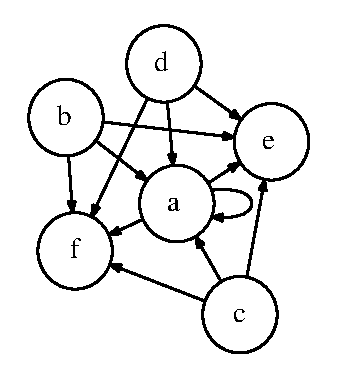
\includegraphics{images/non-reversible-reaction-example.dot.eps}
\end{figure}
supponendo che la specie $a$ appartenente ad entrambi gli
insiemi sia la stessa (ovvero se $\exists a': a = a' \rightarrow id(a) =
id(a') \wedge compart(a) = compart(a')$).

\item data una reazione reversibile $r$ tale che:
  \begin{displaymath}
    \begin{split} 
      reactants(r) &= \{ r_{1}, \ldots, r_{n} \} \\
      products(r) &= \{ p_{1}, \ldots, p_{m} \}
    \end{split}
  \end{displaymath}
  allora il nostro modello sar\`a uguale al grafo che codifica la
  relazione $(reactants(r) \times products(r)) \cup (products(r)
  \times reactants(r))$. Ad esempio, con $reactants(r) = \{ a, b, c, d
  \}$ e $products(r) = \{a, e, f\}$ otteniamo:

\begin{center}
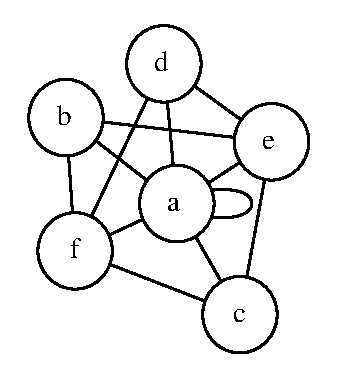
\includegraphics{images/reversible-reaction-example.dot.eps}
\end{center}
supponendo che la specie $a$ appartenente ad entrambi gli
insiemi sia la stessa (ovvero se $\exists a': a = a' \rightarrow id(a) =
id(a') \wedge compart(a) = compart(a')$).

\end{itemize}

Nella prossima sezione descriveremo alcuni dettagli e caratteristiche
di modelli SBML che non sono esplicitamente documentate sul sito
ufficiale (vedi \cite{sbmlOfficialDocumentation}), ma che abbiamo
capito e dedotto utilizzando il concetto di \emph{learning test} (vedi
\cite[p. 136]{beck2003}) implementato con \emph{JUnit}.

\section{Learning SBML tips by tests}

Scrivendo alcuni \emph{learning tests} abbiamo dedotto le seguenti
propriet\`a sui modelli SBML. I seguenti test sono stati esercitati su
una batteria di modelli biologici reali, tutti con esito positivo:
\begin{itemize}
\item sia $r$ una reazione e siano $reactants(r), products(r)$ gli
  insiemi di \emph{reactants} e \emph{products}
  rispettivamente. Questi due insiemi catturano il concetto di insieme
  matematico, ovvero non contengono oggetti duplicati.
\item $\exists r,t \in Reactions: products(t) = reactants(r)$. Questa
  propriet\`a permette di avere continuit\`a tra reazioni, ovvero un
  insiemi di \emph{products} di una reazione $t$ pu\`o essere
  l'insieme di \emph{reactants} di una reazione $r$. Questa
  propriet\`a permette di costruire delle \emph{metabolic pathways}
  composte da quante reazioni si voglia.
\item ogni species deve essere contenuta in un compartment.
\item l'identificatore discrimina le species, ovvero se tentiamo di
  aggiungere al modello due species con lo stesso identificatore, ma
  contenute in compartimenti diversi, allora nel modello viene
  inserita una delle due ma non entrambe, scegliendo in ordine
  cronologico di inserimento
\end{itemize}

\chapter{Theoretical background}
\label{chapter:theoretical-background}

In questo capitolo affronteremo gli algoritmi alla base delle
implementazioni da un punto di vista teorico. Vedremo la tecnica di
visita del grafo che abbiamo adottato e un \emph{survey} degli
algoritmi per il calcolo delle componenti fortemente connesse.

Prima di questi studi introduciamo formalmente cosa \`e una
\emph{story} e cosa significa \emph{telling them}.

\section{"Telling stories" characterization}


\section{DFS search}

La ricerca (o visita) di un grafo \`e una procedura che rivela molte
informazioni sulla sua struttura e molte implementazioni richiedono
tempo lineare.

Prima di descrivere in particolare la ricerca oggetto di questa
sezione, diamo una breve descrizione del problema pi\`u generico,
ovvero di cosa significa visitare un grafo. 

\subsection{The search concept}

Sia $G$ il grafo che vogliamo visitare. Inizialmente tutti i vertici
che compongono il grafo sono sconosciuti, nessuno di essi \`e stato
\emph{esplorato}. Iniziamo da un vertice e seguiamo uno dei suoi
archi, che porter\`a ad un nuovo vertice. Continuiamo ad applicare
questa tecnica: quando arriviamo ad un vertice selezioniamo un arco
non ancora percorso, uscente da vertici gi\`a conosciuti. Percorrendo
l'arco che volta volta viene selezionato, si arriva in un vertice che
possiamo aver gi\`a visitato oppure no. Quando non \`e possibile
selezionare nessun arco non ancora percorso uscente da vertici gi\`a
visitati, allora si seleziona un vertice non ancora selezionato e si
riapplica la tecnica descritta precedentemente.

Come si capisce dal paragrafo precedente, la visita mira ad
identificare un insieme di vertici del grafo a partire da un vertice
dato in cui la visita ha inizio.

\subsection{\emph{Depth First} strategy as maze solver}
Nella precedente sezione abbiamo dato l'idea alla base di una
visita. Vi sono molte strategie che differenziano una visita
dall'altra, ognuna caratterizzata dalla modalit\`a con cui si sceglie
il prossimo arco da percorrere.

La ricerca \emph{Depth First Search} \`e caratterizzata dalla seguente
strategia: \emph{nella selezione del prossimo arco da percorrere,
  scegliere un arco uscente non ancora percorso dal vertice pi\`u
  recentemente esplorato}.

L'insieme dei vertici \emph{pi\`u recentemente esplorati} pu\`o essere
mantenuto in uno \emph{stack}.

Per capire meglio il pattern di questa tecnica supponiamo di iniziare
la visita dal vertice $v$. Prima $v$ viene visitato, poi il suo primo
vicino $v_{1}$ viene scelto e si percorre l'arco $(v, v_{1})$. Adesso
$v_{1}$ viene visitato e si riapplica lo stesso metodo al vicinato di
$v_{1}$. Solo quando tutti i vertici nel vicinato di $v_{1}$ sono
visitati \`e possibile continuare ad esplorare il secondo vicino
$v_{2}$ di $v$ (\`e possibile che $v_{2}$ venga visitato durante
l'esplorazione di $v_{1}$, in questo caso non \`e necessaria nessuna
operazione su $v_{2}$).

L'aggettivo \emph{Depth First} cattura l'idea che la ricerca procede
in profondit\`a, allontanandosi sempre pi\`u dal punto di partenza,
spostandosi da un vertice al un vicino di tale vertice, al vicino del
vicino di tale vertice e cos\`i via, tornando indietro solo quando si
raggiunge un vertice il cui vicinato \`e completamente esplorato,
oppure che tale vicinato sia vuoto.

\begin{paragraph}{maze problem solver}
  Papadimitriou, in \footnote{aggiungere qui riferimento bibliografico
    a Algorithms, pag 83}, vede questa ricerca come un algoritmo per
  risolvere un labirinto, identificandone le idee principali che
  abbbiamo espresso in forma diversa nei precedenti paragrafi:
\begin{quotation}
  [...] the reachability problem is rather like exploring a
  labyrinth[...], a careless choice of passage might lead you around
  in circles or might cause you to return to passages that you
  previously saw but did not investigate.[...] Everybody knows that
  all you need to explore a labyrinth is a ball of string and a piece
  of chalk. The chalk prevents looping, the string always takes you
  back...
\end{quotation}
Riportando questa idea su quanto detto sopra, il concetto di vertice
\emph{esplorato} corrisponde al \emph{chalk}, mentre l'insieme di
vertici \emph{pi\`u recentemente esplorati} corrisponde a \emph{ball
  of string}.
\end{paragraph}

\begin{paragraph}{Pseudocode and complexity}
  Formalizziamo la visita \emph{Depth First Search} nel seguente
  pseudo codice:
  \begin{lstlisting}
    procedure DFS(G = (V, E))
      for all v in V:
        visited(v) = false

      for all v in V:
        if not visited(v):explore(v, E)

    procedure explore(v, E):
      visited(v) = true
      previsit(v)
      for each edge (v, u) in E:
        if not visited(u): explore(u)
      postvisit(v)
  \end{lstlisting}
\end{paragraph}
Facciamo una breve analisi della complessit\`a. La prima osservazione
da fare \`e che ogni vertice viene esaminato una e una sola volta
grazie all'array \emph{visited}. Durante l'esplorazione di un vertice
si spende una quantit\`a costante per settare il vertice come visitato
e per le due invocazioni delle funzioni \emph{previsit,
  postvisit}. Per quanto riguarda invece la scansione del vicinato,
abbiamo per ogni vertice un tempo impiegato diverso, per questo motivo
consideriamo l'intero insieme di archi in una sola volta. Ogni arco
verr\`a visitato una e una sola nel caso in cui il grafo in input sia
orientato, altrimenti due volte nel caso in cui il grafo in input sia
non orientato. Segue che il tempo impiegato dalla visita \`e $O(|V| +
|E|)$, lineare nella lunghezza dell'input.

Un ultima osservazione sulle due operazioni \emph{previsit,
  postvisit}. Se il grafo in input $G$ \`e un albero allora se
utilizziamo solo $previsit$ il risultato \`e equivalente ad una visita
\emph{prefissa} dell'albero, mentre se utilizziamo solo
\emph{postvisit} otteniamo una visita \emph{postfissa} dell'albero.

\section{Tarjan algorithm}

\chapter{Study}
\label{chapter:study}

In questo capitolo affronteremo le principali forze che abbiamo
utilizzato nella fase progettazione e che ci hanno permesso di dar
forma alle nostre idee. 

Faremo riferimento ad una tecnica che non \`e stato possibili
applicare nella fase di progettazione, cercheremo di descrivere gli
obiettivi e i risultati effettivi ottenuti e, infine, descriveremo lo
schema architetturale alla base di tutta l'implementazione,
introducendo l'idea della \emph{pipeline}.

\section{ICONIX method difficult to see here}
Durante il corso di \emph{Tecniche di programmazione} ho avuto
opportunit\`a di sviluppare un progetto utilizzando una metodologia
sviluppata da Doug Rosemberg e Matt Stephens, chiamata \emph{ICONIX},
la quale mira ad improntare lo sviluppo partendo da dei documenti di
specifica del comportamento e, in modo iterativo, raffinarli (in
seguito a successive convalidazioni) in modo da produrre dei documenti
tecnici di pi\`u basso livello, contenenti tutte le informazioni
richieste per una implementazione chiara e precisa \footnote{Su questa
  tecnica ho avuto modo di discutere e avere delle correzioni da due
  colleghi, Arash Tavallay e Emanuele Conti, che ringrazio molto per i
  loro consigli}.

Riporto un passo preso dal volume che introduce
\emph{ICONIX}\footnote{aggiungere qui riferimento bibliografico a USe
  Case Driven, pag. 50} che ritengo catturi le idee chiavi da usare
come punto di partenza:
\begin{quotation}
  \textbf{Don't Forget the Rainy-Day}: Scenarios when you're writing
  your use cases, write them in such a way that your efforts are
  focused on capturing your users' actions and the associated system
  responses. As you'll see, use case modeling involves analyzing both
  the basic course (a user's typical "sunny-day" usage of the system;
  often thought of as 90\% of the behavior) and the alternate courses
  (the other 10\% of the system functionality, consisting of
  "rainy-day" scenarios of the way in which the user interacts with
  the system; in other words, what happens when things go wrong, or
  when the user tries some infrequently used feature of the
  program). If you capture all of this in your use cases, you have the
  vast majority of the system specced out.
\end{quotation}

Nonostante ci siano degli aspetti che non condivido appieno del metodo
(in particolare sui \emph{domain model}, come il lettore si render\`a
conto al termine delle prime sezioni del capitolo
\ref{chapter:implementation}), ci sono comunque dei punti di forza (in
particolare i \emph{robustness diagrams}) che avrei avuto piacere
utilizzare durante questo lavoro, di cui invece non ho potuto giovarne
dei vantaggi.

La maggior difficolt\`a che ho trovato nello stilare \emph{use-case}
seguendo le linee di \emph{ICONIX} sono dovute al fatto che il mio
lavoro non ha una natura interattiva (anche se si potrebbe obiettare
che l'attore \emph{user} sia a sua volta un programma e non un utente
umano) e applicare la regola \emph{two-paragraph rule}
\footnote{aggiungere riferimento bibliografico al volume Use Case
  Driven, pag. 52} nella descrizione degli use-case non portava
vantaggi nella specifica delle mie idee.

Per un esempio di quello che si potrebbe ottenere utilizzando tale
regola, non applicato ad \emph{toy examples}, bensi ad un progetto
reale, si rimanda a \footnote{aggiungere qui riferimento bibliografico
  alla tesi di Arash e Ema}.

Per i motivi sopra esposti, nelle prossime sezioni le descrizione
degli use-case non sar\`a molto formale ma avr\`a una forma pi\`u
discorsiva.

\section{Use cases}
\label{section:use-cases}
% \input{domain-model.tex}
\section{L'architettura \emph{pipes and filters}}

In questa sezione descriveremo l'architettura che vogliamo dare al
nostro lavoro, coscienti degli obiettivi espressi nelle precedenti
sezioni e delle loro caratteristiche.

Daremo prima alcune idee prese dagli articoli che hanno introdotto
quest'architettura e, nella seconda parte della sezione, vedremo come
possiamo ``metterle a punto'' nel nostro progetto.

\subsection{Cenni teorici}
Quest'architettura \`e molto usata nella pratica e vi \`e molta
letteratura da cui poter attingere, pensiamo per\`o che tornare alle
sorgenti che per prime hanno permesso la sua diffusione sia di
notevole importanza prima di analizzare le varianti e gli studi
successivi.

I volumi da cui ho studiato sono quello del Buschmann \cite{POSA} e
dalla miscellanea di Coplien e Schmidt \cite{PLOPD}.

\subsubsection{Schema classico}
Nella testata che descrive il pattern in \cite{POSA}, pagina 53,
compare:
\begin{quotation}
  The \emph{Pipes and Filters} architectural pattern provides a
  structure for systems that process a stream of data. Each processing
  step is encapsulated in a filter component. Data is passed through
  pipes between adjacent filters. Recombining filters allows you to
  build families or related systems.
\end{quotation}
L'idea alla base di questo pattern \`e il principio \emph{separation
  of concerns}. Quello che si vuole fare \`e dividere tutte le
responsabilit\`a del sistema in sotto problemi, ognuno dei quali pu\`o
essere implementato con una componente software tale che \emph{non
  abbia dipendenze} comportamentali dalle altre componenti (non \`e
client di nessun'altra, non vi \`e delega di comportamento) e che
\emph{coopera} con le altre componenti usando l'output di una
componente come input per un'altra.

\`E interessante quello che aggiungono Coplien e Schmidt in
\cite{PLOPD}, pagina 431:
\begin{quotation}
  Usually, transformation of input data is done locally and
  incrementally, so that output may begin before the input is
  completely read. This means that a filter may start to work as soon
  as its predecessor produces its first result.
\end{quotation}
Quest'idea \`e molto importante se vogliamo introdurre un grado
maggiore di parallelismo nel sistema oppure distribuire la
computazione. Nel nostro lavoro questo non \`e stato possibile farlo,
in quanto le computazioni che abbiamo incapsulato nei nostri filtri
non permettono di produrre un output che possa ritenersi un
semilavorato, pronto per essere raffinato dal filtro successivo.

\subsubsection{Conseguenze sull'uso dei filtri}
Riportiamo ancora un'osservazione fatta in \cite{PLOPD}, pagina 431:
\begin{quotation}
  To preserve the independence of the framework's components, filters
  may not share a state. The only way to put the results of different
  filters together is to organize some of them into a sequence such
  that certain filters perform further transformations on the outputs
  of others. In addition, a filter should not know the identity of the
  filters preceding or following it in the computation sequence.
\end{quotation}
Lo funzionalit\`a \ref{subsection:use-case-tarjan} \`e in un certo
senso quello che Coplien identifica nella frase ``...\emph{certain
  filters perform further transformations...}'' per la funzionalit\`a
\ref{subsection:use-case-result-viewer}, in quanto quest'ultima assume
di lavorare su un grafo che sia la minimizzazione di un grafo
utilizzando un algoritmo per la ricerca delle componenti fortemente
connesse.

Aver introdotto formalmente il concetto di filtro come astrazione \`e
stato molto vantaggioso in quanto ogni computazione, sia effettiva che
di "adattamento", pu\`o essere trattata indipendentemente e in modo
trasparente alla stregua delle altre.

\subsubsection{Conseguenze sull'uso delle pipes}
Riporto ancora da Coplien, pagina 432:
\begin{quotation}
  Two principally different possibilities exist for the realization of
  pipes: pipes may simply be links between filters (such as message
  calls) or they may be separate components (such as data repositories
  or sensors). A pipe's only responsibility is to transmit data
  between filters, eventually by converting their format from the one
  produced by their sender to the one required by their receiver.
\end{quotation}
Nel nostro lavoro non abbiamo avuto bisogno della complessit\`a di
modellare veri e propri oggetti \emph{pipe} in quanto, come vedremo
nella prossima sezione, non \`e necessario adattare il formato
dell'input per coppie diverse di filtri, responsabilit\`a di oggetti
\emph{pipe}. Abbiamo quindi scelto la modalit\`a ``\emph{links between
  filters}''.

\subsection{Implementazione in questo progetto}
L'implementazione dell'architettura \emph{pipes and filters} in questo
progetto ha cercato di prendere spunto da quanto detto nella sezione
precedente ma allo stesso tempo ha delle caratteristiche che la
distinguono dalla linea introdotta.

Abbiamo introdotto la classe \emph{PipeFilter} per modellare il
concetto di \emph{filtro} e, come sua propriet\`a, un riferimento al
filtro successivo, per modellare il concetto di \emph{pipe}.

Inoltre possiamo vedere la \emph{pipeline} come una coda di filtri,
dove il primo filtro ad essere inserito nella pipeline \`e il primo ad
essere eseguito. Utilizzando la terminologia usata da Buschmann, la
nostra implementazione ricade nello scenario ``\emph{pull pipeline}'',
dove la computazione viene innescata dalla richiesta di un client.

Non vi \`e bisogno di logica di conversione dell'output di un filtro
per esser trattato come input per un altro, in quanto ogni filtro
lavora con l'astrazione \emph{OurModel}, anche se avremo comportamento
diverso in base al tipo di oggetti \emph{Vertex} contenuti all'interno
dell'input\footnote{aggiungere qui riferimento all'appendice
  riguardante i precedenti concetti}.

La precedente osservazione potrebbe indurre il lettore a pensare alla
nostra architettura non tanto come una pipeline, quanto come un
sistema di decoratori (vedi pattern \emph{Decorator} in
\cite{SmalltalkCompanion98}). Questa interpretazione non \`e errata,
anzi crediamo che indebolire il requisito di stabilire un ordinamento
rigido dei filtri presente nel pattern \emph{pipeline} originale, a
favore di maggior dinamicit\`a e trasparenza sul formato di
input/output, porti ad una soluzione che sarebbe stato sufficiente
implementare con un tipico schema con decoratori.


\chapter{Implementation}
\label{chapter:implementation}
In questo capitolo daremo delle informazioni di alto livello
riguardanti l'implementazione dei concetti descritti nel capitolo
\ref{chapter:study}, descrivendo la metodologia di sviluppo
utilizzata, quali paradigmi e stili di programmazione sono alla base
delle implementazioni e un breve overview sulle funzionalit\`a
incapsulate in ogni \emph{package} della libreria.

\section{Development methodology}

In questa sezione descriver\`o la metodologia di sviluppo che ho
adottato per sviluppare la fase di implementazione.

Ho sempre avuto molta curiosit\`a sui metodi \emph{agile} e,
soprattutto, sulla metodo \emph{Test Driven Development}. Non ho mai
avuto opportunit\`a di affrontare un progetto usando queste linee idee
e ho pensato che questo lavoro potesse essere un buon banco di prova.

Il volume su cui ho cercato di apprendere questa tecnica \`e
\footnote{aggiungere riferimento bibliografico qui al volume scritto
  per intero} \emph{Test Driven Development: By Example} scritto da
Kent Beck. In questo scritto vi sono molti esempi, scritti usando il
linguaggio di programmazione \emph{Java}, anche se le idee di avere
test automatici per assicurare la qualit\`a del codice erano gi\`a
state battute in \emph{Lisp} e, dallo stesso Beck, in
\emph{Smalltalk}.

Riporto la prima frase della prefazione:
\begin{quotation}
  \emph{Clean code that works}, in Ron Jeffries' pithy phrase, is the
  goal of Test-Driven Development. Clean code that works is a
  worthwhile goal for a whole bunch of reasons...
\end{quotation}
Non posso certo dire che le mie implementazioni soddisfino la
citazione precedente (almeno per la parte \emph{that works}), per\`o
aver guidato l'intero sviluppo tramite test \`e stata una esperienza
molto istruttiva, di cui sono soddisfatto.

Nelle prossime sezioni descrivo come i \emph{tests} sono stati di
grande aiuto durante il lavoro.

\subsection{Learning tests}
Questo tipo di test sono stati scritti soprattutto durante i primi
momenti di sviluppo, e hanno avuto l'obiettivo di
familiarizzare l'utilizzo della libreria \emph{JSBML}. 

La documentazione fornita \`e estesa e ben dettagliata, per\`o ci
sono stati degli aspetti che senza aver esercitato alcuni test non era
possibile studiarli a priori.

Per questi tests ho dedicato un package dedicato, in modo da
fattorizzare in un unico contenitore tutta la logica che ho avuto
bisogno per chiarire tutti gli aspetti necessari all'avanzamento del
mio lavoro.

In \footnote{aggiungere qui riferimento bibliografico a TDD, pag 136}
viene spiegato questo "pattern" e un aspetto che non ho potuto
sperimentare direttamente in questo sviluppo, ma che penso sia
interessante notare. Se viene rilasciata una nuova versione della
libreria \emph{JSBML} abbiamo il grande vantaggio di avere delle
asserzioni che verificano i concetti che abbiamo utilizzato come
dipendenze per il nostro lavoro. Siamo interessati che nessuna di
queste \emph{assert} sia violata dal nuovo rilascio. 

Senza questi test avremo dovuto provare il software manualmente per
controllare che il comportamento non sia cambiato. Avendoli invece,
\`e sufficiente far "correre" di nuovo tutta la batteria per
assicurare che i concetti su cui ci siamo basati non abbiano subito
modifiche.

\subsection{Pros}
Il maggior vantaggio che ho avuto utilizzando questa metodologia \`e
stato di poter pensare ad una funzionalit\`a vestendo due
"cappelli". Dapprima ho potuto concentrarmi sul comportamento che
desideravo, quindi poter pensare solo il sistema di messaggi che i
miei oggetti si sarebbero scambiati (e questo corrisponde alla fase
\emph{test-first}), creando un \emph{test method} per catturare
l'idea.

Quando vedevo il nuovo test fallire, ho potuto dedicarmi
all'implementazione necessaria per passare il test. 

A differenza di quanto suggerisce Beck, non ho quasi mai applicato il
pattern \emph{Fake it, ('Til you make it)} \footnote{aggiungere qui
  riferimento a TDD, pag. 151}, in modo da arrivare subito alla
\emph{green bar} e procedere poi alla rimozione dei eventuali
duplicazioni o \emph{code smell} mediante refactoring, perch\`e in
molti casi l'implementazione necessaria per superare il test non era
cosi complessa da dover procedere in \emph{baby step} (usando la
terminologia di Beck).

Forse sono stato un po' troppo prolisso sotto alcuni aspetti: le mie
batterie di test contano un totale di 191 metodi di test. Magari si
sarebbe potuto risparmiare qualcosina, per\`o quasta granularit\`a
fine penso sia stata di aiuto nella fase di superamento del test, la
maggior parte delle volte la logica da implementare non \`e stata
difficoltosa.

\subsection{Cons}
Una nota negativa che ho registrato riguarda il grado di profondit\`a
(se si vuole di precisione) che ho associato ai test pi\`u critici.

Nella parti pi\`u delicate mi sono sempre chiesto se i test scritti
era sufficienti a catturare il comportamento che effettivamente avrei
voluto. In alcuni punti ho dovuto ricorrere al debugger, ma penso che
questo sia accettabile, per aiutarmi a capire se qualche aspetto
necessit\`a di maggior copertura da parte dei metodi di test.

Parte di questi dubbi penso derivino anche della mia non esperienza
riguardo questo metodo.

Un altro punto in cui ho avuto difficolt\`a e che mi distacco da
quello che esprime Beck, riguarda lo stile con cui ho scritto le mie
asserzioni. In \footnote{aggiungere qui riferimento bibliografico a
  TDD, pag. 157}, Beck suggerisce di essere il maggior precisi
possibile nella scrittura di una \emph{assert}, riporto un esempio:
\begin{quotation}
  I've seen assertions like \emph{assertTrue(rectangle.area() !=
    0)}. You could return anything not null and satisfy this test, so
  it isn't very useful. Be specific. If the area should be 50, then
  say that it should be 50: \emph{assertEquals(50, rectangle.area())}.
\end{quotation}
Credendo nei principi espressi nella sezione
\ref{sec:objects-oriented-functional-paradigms}, quindi riducendo
l'uso di metodi accessori, ho avuto difficolt\`a a seguire i consigli
di Beck. Penso per\`o di aver recuperato usando un altra idea che
ritengo molto importante per la scrittura di solidi metodi di test: la
\emph{triangolazione} \footnote{aggiugere qui riferimento
  bibliografico a TDD, pag.153}. 

Questa idea mi ha permesso di utilizzare un approccio molto "chiuso"
per quanto riguarda l'uso di accessori, usando messaggi con lo
stile \emph{isSomethingEquals(...)}, e scrivere lo stesso metodi di
test solidi. Ad esempio:
\begin{lstlisting}
  @Test
  public void matchSpeciesCompartement() {
    Vertex v1 = VertexFactory.makeSimpleVertex();
    Vertex v2 = VertexFactory.makeSimpleVertex();
    Assert.assertNotSame(v1, v2);
    Assert.assertTrue(v1.matchCompartmentWith(v2));
    Assert.assertTrue(v2.matchCompartmentWith(v1));
    Assert.assertFalse(v1.matchSpeciesWith(v2));
    Assert.assertFalse(v2.matchSpeciesWith(v1));
  }
\end{lstlisting}
Usando questo schema, anche se il metodo \emph{matchCompartmentWith()}
invocato sull'oggetto \emph{v1} restituisse un valore fittizio solo
per superare il test, la seguente invocazione su \emph{v2} lo
contraddirrebbe, fallendo il test.


\section{Pure object-oriented and functional programming paradigms}
\label{sec:objects-oriented-functional-paradigms}

Nella prossime sezioni faremo una breve panoramica sui package che
contengono le implementazioni.

\section{Packages' descriptions}
\label{section:packages-descriptions}

Nelle prossime sezioni descriveremo gli oggetti implementati nei
\emph{packages} java. Ogni package verr\`a descritto in una sezione
dedicata, dandone i concetti principali, alcuni diagrammi usando la
notazione \emph{UML} e alcuni dettagli implementativi di interesse ed
eventuali design patterns and coding idioms che hanno aiutato
nell'implementazione.

\subsection{Pacchetto dotInterface}
\label{subsection:dotInterface-package-description}
Questo pacchetto incapsula tutte quelle astrazioni necessarie alla
creazione di un documento compilabile con i motori messi a
disposizione dalla libreria \emph{graphviz}.

\subsubsection*{Funzionalit\`a implementate}

Le funzionalit\`a fornite da questo pacchetto sono le seguenti:
\begin{itemize}
\item definire i contratti fondamentali che codificano le
  responsabilit\`a affinch\`e un oggetto sia esportabile in formato
  dot e, in modo duale, sia capace di esportare in formato dot un
  altro oggetto. Questi due contratti sono le astrazioni pi\`u
  importanti di tutto il pacchetto e sono dipendenze delle classi
  \emph{Vertex} e \emph{OurModel};
\item incapsulare in un'unica classe tutte quelle funzionalit\`a e
  caratteristiche utilizzate durante la generazione dell'output,
  alcune di esse dipendenti dal sistema operativo che ospita la
  \emph{Java Virtual Machine}, ad esempio: il separatore utilizzato
  nei percorsi di file e directory nel file system, posizioni degli
  output della libreria e delle cartelle dove trovare i modelli di
  input;
\item fornire un wrapper per oggetti di tipo \emph{Writer}, che
  permetta di concatenare alla rappresentazione testuale dell'oggetto
  il carattere `;', i due caratteri di \emph{carriege return} e
  \emph{new line} per appendere il prossimo contenuto su una nuova
  linea. Questo agevola la scrittura di documenti dot, nei quali ogni
  linea deve avere una linea propria ed essere terminata da `;'.
\end{itemize}

\subsubsection*{Classi}
Procediamo con ordine nel descrivere le principali classi:

\begin{paragraph}{DotExporter}
  Il contratto \emph{DotExporter} definisce quali sono i messaggi che
  un esportatore deve essere in grado di comprendere per costruire
  documenti in formato dot, lavorando su un grafo codificato con le
  astrazioni di \emph{Vertex} e \emph{OurModel}.

  I messaggi definiti in \emph{DotExporter} riguardano le componenti
  basilari di un grafo che si possono rappresentare graficamente: il
  vertice (con eventuale etichetta esterna al nodo) e l'arco (di cui
  non \`e stato necessario introdurre un'etichetta). Riporto il codice
  per maggior chiarezza:
  \begin{lstlisting}
public interface DotExporter extends DotDocumentPartHandler {
  DotExporter buildVertexDefinition(Vertex vertex);
  DotExporter collectCompleteContent(Writer outputPlugObject);
  DotExporter buildEdgeDefinition(Vertex source, Vertex neighbour);
  DotExporter buildVertexLabelOutsideBoxDefinition(Vertex vertex);
}

public interface DotExportable {
  void acceptExporter(DotExporter exporter);
}

  \end{lstlisting}
  Per non accoppiare in modo forte la modalit\`a di salvataggio
  dell'output nei messaggi dell'interfaccia, ne viene esposto uno che
  ha come argomento un oggetto di tipo \emph{Writer}, appartenente alla
  libreria di \emph{io} fornita in \emph{openjdk}.

  Questo non limita l'insieme di destinazioni dell'output, bens\`i
  lascia aperte molte scelte ed eventuali client del contratto
  \emph{DotExporter} potranno utilizzare i propri oggetti come
  destinazione dell'output, potendoli usare per computazioni
  successive. Nelle nostre implementazioni abbiamo usato quasi sempre
  oggetti di tipo \emph{FileWriter} come destinazioni concrete.
\end{paragraph}

\begin{paragraph}{DotExportable}
  Questo contratto permette di definire quali responsabilit\`a devono
  essere implementate affinch\`e un oggetto sia esportabile in formato
  dot.

  Non \`e un interfaccia molto ricca, ma il solo messaggio
  \emph{acceptExporter} \`e sufficiente per catturare la nostra
  idea. Questa struttura si avvicina molto a quella che viene esposta
  nel pattern \emph{Visitor} in \cite{SmalltalkCompanion98}, anche se
  la nostra implementazione non la ricalca fedelmente: il taglio che
  abbiamo voluto dare alla coppia \emph{DotExporter} e
  \emph{DotExportable} usa lo stesso il \emph{double dispatch}, con la
  differenza di non esporre nel contratto \emph{DotExporter} i metodi
  relativi alle classi concrete di \emph{Vertex}, avendo un solo
  messaggio \emph{buildVertexDefinition} come sopra riportato.
\end{paragraph}





\subsection{Pacchetto JSBMLInterface}
\label{subsection:JSbmlInterface-package-description}
Questo pacchetto contiene le implementazioni dei concetti che
riguardano l'interfacciamento con modelli SBML utilizzando la libreria
\emph{JSBML} (vedi \cite{JSbmlDistribution}).

\subsubsection*{Funzionalit\`a implementate}

Le funzionalit\`a fornite da questo pacchetto sono le seguenti:
\begin{itemize}
\item astrarre dalla libreria \emph{JSBML} e dal suo modello dati. In
  questo modo l'unico contesto del progetto dipendente dalla libreria
  \emph{JSBML} \`e confinato a questo singolo pacchetto e gli altri
  pacchetti non dovranno essere a conoscenza di come viene codificato
  il modello. Usando questa strategia se si vorr\`a sostituire la
  libreria di interfacciamento con modelli SBML, sar\`a necessario
  apportare le modifiche solo in questo pacchetto, lasciando tutto il
  restante codice del progetto inalterato;
\item interpretare il modello fornito dalla libreria \emph{JSBML},
  costruire gli elementi fondamentali del nostro modello dati e
  renderlo disponibile per successive computazioni.
\end{itemize}

\subsubsection*{Classi}
In questo pacchetto la classe principale \`e \emph{Connector}, la
quale incapsula la responsabilit\`a di delegare alla libreria
\emph{JSBML} la lettura di un modello SBML e, successivamente,
interpretare il risultato della lettura per costruire un nostro
modello dati interno, input di successive computazioni.

La parte di interpretazione del modello letto dalla libreria
\emph{JSBML} \`e quella pi\`u interessante in quanto elabora e
seleziona solo quelle informazioni del modello SBML che effettivamente
sono necessarie al nostro lavoro.

Questo procedimento \`e implementato principalmente nel metodo
\emph{readReactions}, il quale permette di costruire un insieme di
vertici a partire da una collezione di reazioni, i quali verranno
usati per costruire il modello di dominio.

\section{Model package}

In questa sezione descriveremo il package \textbf{Model}.

Questo package contiene le implementazioni dei concetti che riguardano
la pi\`u importante e ricca astrazione del concetto di vertice, del
nostro modello di grafo, delle specializzazioni del concetto di
vertice e di due astrazioni legate alla programmazione funzionale.

\subsection{Supplied Abstractions}
\label{subsection:model-supplied-abstractions}
Le astrazioni fornite da questo package sono le seguenti:
\begin{itemize}
\label{itemize:model-supplied-abstraction}
\item fornire l'astrazione di vertice e le sue specializzazioni
  necessarie per implementare gli altri moduli del progetto. Questa
  astrazione pu\`o essere modellata a livello teorico come un
  \emph{abstract data type}, in quanto non siamo interessati che i
  client siano a conoscenza delle specifiche realizzazioni (come
  invece lo sarebbe se fosse stato un \emph{algebraic data type}), ma
  vogliamo usare un approccio trasparente per mantenere flessibile il
  sistema. Le specializzazioni del concetto di vertice che ho
  implementato riguardo il concetto semplice di vertice, di vertice da
  usare in una ricerca \emph{DFS} e nell'algoritmo di Tarjan per la
  ricerca delle componenti fortemente connesse.
\item fornire l'astrazione del grafo, arricchendola con comportamenti
  per poter modificare la struttura del grafo rappresentato e poter
  eseguire delle computazioni su di esso: \`e possibile usare due idee
  prese dal paradigma funzionale per agire sui vertici del grafo ed
  \`e fornita una implementazione dell'algoritmo \emph{DFS}, che espone
  degli \emph{hot spots} in modo da permettere ai client di avere
  gi\`a implementata la struttura dell'algoritmo, fornendo solo il
  comportamento specifico di interesse.
\item nascondere tutti i tipi che implementano i concetti astratti ai
  client di questo package, in modo da utilizzare le astrazioni
  mediante interfaccie e non accoppiando i client con specifiche
  realizzazioni attraverso delle factory 
\item interfacciare le astrazioni di vertice e grafo con gli oggetti
  definiti nel package \emph{DotInterface}, per permettere una
  rappresentazione grafica che cattura le idee definite nell'articolo
  \cite{tellingStories}
\end{itemize}

\subsection{Class diagram}
Il diagramma rappresentato in figura
\ref{fig:vertex-abstraction-interfaces} rappresenta le interfaccie
introdotte in questo package. Procediamo con ordine nel descrivere le
idee principali catturate in ogni contratto:

\begin{figure}
  \centering
  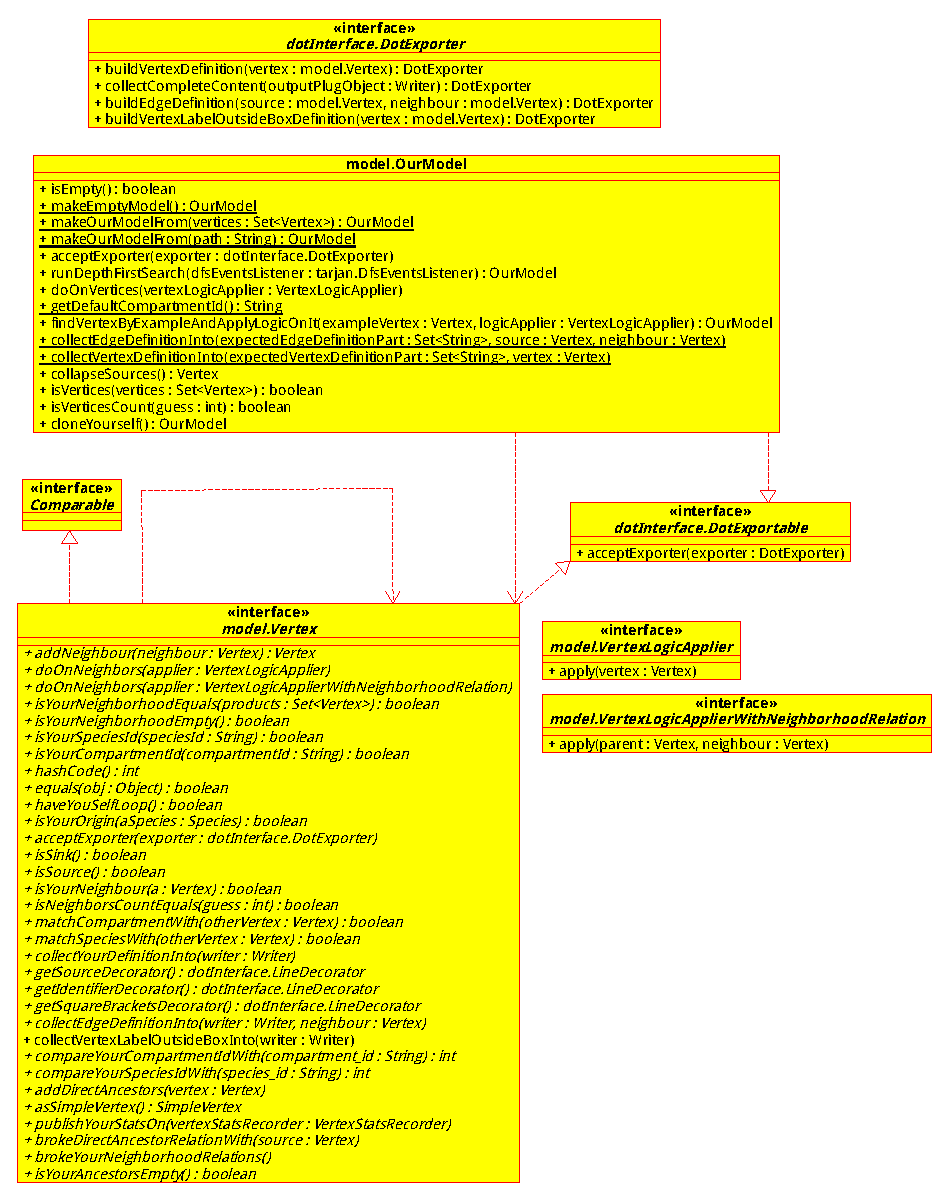
\includegraphics{packages/vertex-interface-class-diagram.eps}
  \caption{Vertex abstraction interfaces}
  \label{fig:vertex-abstraction-interfaces}
\end{figure}

\begin{paragraph}{Vertex}

  L'interfaccia \emph{Vertex} \`e l'astrazione principale dell'intera
  libreria ed \`e molto ricca di contenuto.  Tramite \emph{Vertex}
  possiamo richiedere ad un valido implementatore, di gestire le
  informazioni sul vicinato di un vertice, dando la possibilit\`a sia
  di aggiungere vicini che predecessori (quindi modelliamo sia una
  lista di adiacenza, sia una lista di incidenza). Questo ci permette
  di avere un costo nell'ordine $O(m + n)$ dove $m$ \`e il numero
  totali di archi presenti nel grafo codificato nel nostro modello ed
  $n$ \`e invece il numero di nodi dello stesso. Inoltre, per poter
  collassare le sorgenti in una unica\footnote{aggiungere qui
    riferimento alla descrizione del relativo use case}, \`e possibile
  richiedere la "rottura" della relazione di vicinato per poter
  successivamente cancellare il vertice dal grafo, senza lasciare
  coppie nell'insieme degli archi $E$ che contengono nodi sorgente
  rimossi.

  \emph{Vertex} permette di richiedere informazioni sulle
  caratteristiche del vertice, ad esempio se un vertice \`e sorgente o
  pozzo, qual \`e il suo vicinato, quali sono le informazioni che lo
  distinguono (riferite alla \emph{species} e al \emph{compartment}
  recuperate dal modello SBML di origine). Molti di questi metodi sono
  utilizzati soprattutto nei metodi di unit testing e hanno una firma
  che rispetta i concetti espressi nella sezione
  \ref{sec:objects-oriented-functional-paradigms}\footnote{in questa
    sezione descrivere perche si e' evitato metodi di get e set in
    benificio di metodi della forma is...()}.

  Tramite questo contratto possiamo interfacciarci con le
  implementazioni definite nel package
  \emph{dotInterface}\footnote{aggiungere qui collegamento con
    nameref}, richiedendo di poter accettare un esportatore per
  costruire un documento in formato \emph{dot}, fornendo gli oggetti
  necessari per la corretta formattazione delle informazioni
  incapsulate nell'oggetto che implementa il contratto
  \emph{Vertex}. Utilizzando solo contratti, siamo in grado di avere
  questi due comportamenti \emph{loosesly coupled}, in quanto
  cambiamenti agli effettivi implementatori dei due contratti, non
  comportano cambiamenti ai metodi definiti nelle interfaccie.

  Nel precedente paragrafo abbiamo richiesto la possibilit\`a di
  generare un documento grafico (si creano rappresentazioni del grafo
  in formato \emph{svg}), ma \`e possibile richiedere anche delle
  informazioni di carattere testuale dalle quali \`e possibile capire
  meglio la struttura del grafo (sia di un grafo a cui applichiamo
  l'algoritmo di Tarjan e non) attraverso una rappresentazione
  tabulare. Questo comportamento \`e implementato dalla classe
  \emph{VertexStatsRecorder}, dipendenza di questo contratto.

  Una propriet\`a che questo contratto richiede \`e quella di
  riscrivere i metodi \emph{equals} e \emph{hashCode} in modo che
  tutti gli oggetti implementatori di questa interfaccia possano
  essere trattati come \emph{value objects}, non distinguendoli per
  riferimento in memoria (implementazione di default del metodo
  \emph{equals} fornito da \emph{openjdk}), bensi dalle informazioni
  che questi incapsulano (e quindi poter usare \emph{late-binding} ed
  avere comportamento polimorfo in base all'oggetto che riceve i
  suddetti messaggi). Abbiamo effettuato questa scelta in modo da
  poter creare implementatori di \emph{Vertex} all'occorrenza con le
  stesse caratteristiche, senza dover gestire una struttura dati per
  la memorizzazione e la ricerca dell' unico oggetto creato.

  Come ultima propriet\`a, questo contratto impone una relazione
  d'ordine totale sull'insieme degli implementatori, in modo da
  rendere gli algoritmi deterministici nel momento di selezione di
  vertici. Questo \`e stato utile per la stesura dei metodi di unit
  testing.

\end{paragraph}

\begin{paragraph}{OurModel}
  La classe concreta \emph{OurModel} cattura il concetto di grafo da
  utilizzare come modello di dominio per le computazioni descritte nel
  capitolo \ref{chapter:study}.

  La prima responsabilit\`a di \emph{OurModel} \`e quella di fornire
  il comportamento per la costruzione del modello in diverse
  modalit\`a: costruire un modello a partire da un insieme di vertici
  gi\`a costruiti (e, quindi, con le relazioni di vicinato gi\`a
  fissate), oppure a partire da un modello SBML esistente in una path
  del file system.

  Questa classe non solo permette di poter manipolare e rappresentare
  in un "tutt'uno" un grafo, ma espone dei comportamenti fondamentali
  per l'implementazione dei concetti descritti nel capitolo
  \ref{chapter:theoretical-background}.

  Viene fornita la logica per compattare le sorgenti in una unica,
  restituendo una nuova istanza di grafo con la struttura richiesta,
  lasciando immutato il modello di input, dando la possibilit\`a di
  poter continuare ad inviare messaggi al modello originale.

  Un altra importante astrazione che utilizza uno stile funzionale
  permette di poter applicare un comportamento definito dal client di
  \emph{OurModel} su ogni vertice in esso contenuto. Questo \`e stato
  un vero punto di forza che ci ha permesso di aver un codice pulito,
  mantenibile e orientato al testing.

  L'ultimo comportamento che merita attenzione \`e quello di
  templetizzare l'algoritmo di \emph{DFS}, introducendo degli
  \emph{hot spots} sui quali \`e possibile "customizzare" il
  comportamento della ricerca ed implementare delle sue
  varianti. Quelle che abbiamo implementato in questo lavoro sono
  strettamente quelle definite nel capitolo
  \ref{chapter:theoretical-background}, ma questo non limita un
  utilizzatore della libreria di definire il proprio comportamento e
  di usare l'implementazione della ricerca per algoritmi non trattati
  in questo documento.

\end{paragraph}

\begin{paragraph}{Vertex implementors}
  Abbiamo molti comportamenti diversi che vogliamo poter utilizzare
  come istanze dell'astrazione definita dal contratto
  \emph{Vertex}. Il vantaggio di aver implementato il codice
  riferendosi sempre al contratto e non alle singole caratterizzazioni
  ci ha dato l'enorme vantaggio di poter essere trasparenti e poter
  interscambiare questi aspetti specificando solo nel rispettivi
  contesti quale comportamento si preferiva utilizzare, lasciando
  completamente immutato il codice che invece implementa i vari
  algoritmi.

  In questo paragrafo enumeriamo quali sono le caratterizzazioni (il
  \emph{Vector of changes} come viene chiamato da Bruce Eckel in
  \footnote{aggiungere qui il riferimento bibliografico a Thinking in
    Patterns}) e alcune loro propriet\`a.

  La prima caratterizzazione introdotta \`e stata \emph{SimpleVertex},
  la quale cattura il comportamento di un vertice "normale", ovvero
  l'implementazione pi\`u semplice possibile del contratto. Anche se
  questa pu\`o sembrare scontata, invece \`e il building-block
  utilizzato, pi\`u o meno indirettamente, da caratterizzazioni pi\`u
  complesse. Come vedremo \footnote{nella sezione dei patterns
    inserire un paragrafo sulla comodit\`a di utilizzare i wrapper per
    evitare il problema della fragile base class, fare riferimento
    anche al libro di Josch Block}, queste caratterizzazioni avanzate
  sono dei \emph{wrapper} che delegano parte del comportamento alla
  caratterizzazione \emph{SimpleVertex} e ridefiniscono solo il
  comportamento che differisce da quest'ultima.

  La seconda caratterizzazione introdotta \`e stata
  \emph{DfsWrapperVertex}, la quale permette di associare l'analogo di
  un "timestamp" nel momento in cui la ricerca visita un vertice e nel
  momento in cui la visita abbandona il vertice. Questo ci ha permesso
  di produrre una rappresentazione simile a quella che
  \emph{Papadimitriou} propone nel suo volume \footnote{aggiungere qui
    il riferimento bibliografico al volume di Algorithms e alle pagine
    in cui si evidenzia la coppia di interi} ed analizzata nel
  capitolo \ref{chapter:study}.

  La terza caratterizzazione introdotta \`e stata
  \emph{ConnectedComponentWrapperVertex}, in coppia con
  \emph{TarjanWrapperVertex}. Queste due caratterizzazioni permettono
  di implementare in modo puramente orientato agli oggetti l'algoritmo
  di \emph{Tarjan} per la ricerca delle componenti fortemente
  connesse. In particolare \emph{ConnectedComponentWrapperVertex}
  cattura la responsabilit\`a di rappresentare una componente
  fortemente connessa e manipolare l'insieme di nodi del grafo
  originario che la individuano (il lifetime di questa
  caratterizzazione \`e relativo alla parte finale e di utilizzo del
  grafo prodotto dalla minimizzazione), mentre
  \emph{TarjanWrapperVertex} cattura la responsabilit\`a di mantenere
  la relazione di vicinato tra componenti fortemente connesse (il
  lifetime di questa caratterizzazione \`e soprattutto relativo
  all'esecuzione dell'algoritmo). Inoltre, per poter sviluppare un
  piccolo programmetto per la visualizzazione di semplici statistiche
  come descritto nel capitolo \ref{chapter:study}, abbiamo introdotto
  l'astrazione \emph{ConnectedComponentInfoRecorder}.

  Inoltre, anche se sono classi astratte e quindi non immediatamente
  istanziabili, abbiamo introdotto \emph{VertexWithLabelWrapperVertex}
  per dare la possbilit\`a di rappresentare una etichetta sopra alla
  rappresentazione di un nodo nella generazione dell'output
  grafico. Questo comportamento \`e possibile utilizzarlo in modo
  trasparente e permette di fattorizzare e non mischiare nello stesso
  file sorgente (e quindi in una stessa classe) il codice che
  implementa la decorazione e il codice che implementa la particolare
  caratterizzazione del contratto \emph{Vertex}.

  Tutte le precedenti caratterizzazioni sono nascoste ai client del
  contratto \emph{Vertex} dalla factory \emph{VertexFactory} che
  espone metodi statici per poter costruire oggetti che implementano
  il contratto ma avere il codice sorgente il meno accoppiato
  possibile (questa modalit\`a di creazione implica che abbiamo
  pensato il contratto \emph{Vertex} come un vero e proprio
  \emph{abstract data type}).
\end{paragraph}


\subsection{Pacchetto Piping}
\label{subsection:piping-package-description}
Questo pacchetto contiene le implementazioni che permettono di
assemblare una \emph{pipeline}, attraverso la composizione di un
numero quanto si voglia di filtri. 

\subsubsection*{Funzionalit\`a implementate}

Le funzionalit\`a fornite da questo pacchetto sono le seguenti:
\begin{itemize}
\item definire un \emph{template} di filtro, componente atomica per la
  composizione di una \emph{pipeline}. Questo template codifica il
  comportamento necessario affinch\'e possa essere combinato,
  lasciando all'implementatore il compito di sviluppare la logica che
  caratterizza il filtro che st\`a modellando;
\item fornire un insieme di filtri gi\`a implementati necessari alla
  realizzazione delle funzionalit\`a descritte nella Sezione
  \ref{section:use-cases};
\item catturare ed esporre il concetto di \emph{listener}, mediante il
  quale \`e possibile gestire degli eventi che avvengono durante la
  computazione. \`E possibile assemblare la propria pipeline ed,
  attraverso un listener, eseguire non solo le trasformazioni che
  questa produce, ma anche della logica aggiuntiva all'accadere di
  determinati eventi. Questo strumento permette di essere ortogonali
  alla pipeline ed aver maggior controllo sull'intera computazione.
\end{itemize}

\subsubsection*{Classi}
Procediamo con ordine nel descrivere le idee principali catturate
dalle seguenti classi:

\begin{paragraph}{PipeFilter}
  Abbiamo cercato di formalizzare in modo preciso la pi\`u piccola
  unit\`a atomica capace di eseguire una computazione all'interno di
  una sequenza pi\`u grande, portandoci a definire la classe
  \emph{PipeFilter}: introducendola possiamo rendere il codice
  flessibile e trasparente, nonch\'e pi\`u facile da implementare.

  Questa classe, come abbiamo detto nei paragrafi precedenti, in
  realt\`a rappresenta solo un \emph{template} del concetto di filtro
  e non esegue una trasformazione definita sull'istanza di
  input. Usandola \`e possibile assemblare una sequenza di filtri, ed
  eseguire la computazione propagando la richiesta di esecuzione a
  tutti i filtri che si sono assemblati.

  Quello appena detto \`e stato implementato dando a \emph{PipeFilter}
  una struttura ricorsiva: ad esempio per costruire una pipeline con
  due filtri \`e sufficiente costruirli, fissare la relazione di
  precedenza che identifica la pipeline ed invocare la richiesta di
  esecuzione sull'ultimo filtro. Tale filtro, ricevendo la richiesta,
  controlla se il filtro che lo precede esiste: se si, delega la
  richiesta di esecuzione e si riapplica questo procedimento in modo
  ricorsivo, altrimenti esegue la trasformazione per cui \`e stato
  creato. Inoltre, sempre sfruttando la struttura ricorsiva di
  \emph{PipeFilter}, \`e possibile comporre una pipeline i cui filtri
  sono a loro volta pipeline.

  Ogni filtro lavora su un grafo in input, apporta le modifiche che
  implementa e restituisce in output il grafo trasformato. Questa
  trasformazione da grafi a grafi permette di non avere complessit\`a
  aggiuntiva per quanto riguarda la coerenza dei formati di
  input/output tra filtri adiacenti.
\end{paragraph}

\begin{paragraph}{Implementazioni di PipeFilter}
  Come abbiamo detto, \emph{PipeFilter} rappresenta solo un
  \emph{template}: il comportamento che vogliamo dare ad ogni filtro
  deve essere codificato in una classe concreta che "completa" tale
  template. In realt\`a non \`e molto il lavoro che si lascia da
  scrivere: per completare il template \`e sufficiente implementare un
  metodo astratto, che ha come parametri il grafo di input e deve
  ritornare un grafo utilizzato come input per il filtro successivo.

  Il primo filtro concreto che abbiamo introdotto \`e stato
  \emph{PrinterPipeFilter}, il quale produce una rappresentazione
  grafica compilando un documento \emph{dot}: per adempiere a questo
  compito, costruisce un oggetto di tipo \emph{DotExporter} nel quale,
  durante la visita del grafo, colleziona le informazioni necessarie
  per costruire il documento da compilare. Questo filtro non apporta
  nessuna trasformazione al grafo di input e lo restituisce cos\`i
  come lo ha ricevuto.

  Il secondo filtro concreto che abbiamo introdotto \`e stato
  \emph{DfsPipeFilter}, il quale esegue una visita in profondit\`a del
  grafo in input e ritorna un grafo il cui insieme di archi \`e
  composto da tutti gli archi percorsi dalla visita. Concatenando un
  filtro di tipo \emph{PrinterPipeFilter} sar\`a possibile
  visualizzare la foresta di alberi \emph{DFS} rappresentante la
  visita eseguita.

  Il terzo filtro concreto che abbiamo introdotto \`e stato
  \emph{TarjanPipeFilter}, il quale ricerca le componenti fortemente
  connesse sul grafo di input e restituisce un nuovo \emph{DAG}
  composto dalle componenti identificate. \`E importante notare che
  programmando ``per interfacce'', il grafo prodotto da questo filtro
  non ha come vertici dei \emph{SimpleVertex}, bens\`i degli oggetti
  che caratterizzano le componenti fortemente connesse. In questo modo
  possiamo continuare ad inviare gli stessi messaggi che possiamo
  inviare ad un oggetto di tipo \emph{SimpleVertex}, ma ottenere un
  comportamento diverso, senza modificare il codice che implementa il
  modello di dominio.

  Il quarto filtro concreto che abbiamo introdotto \`e stato
  \emph{SourcesCollapserPipeFilter}, il quale permette di collassare
  tutte le sorgenti ed introdurne una nuova ed unica. Il nuovo grafo
  viene restituito per eventuali computazioni successive.

  Gli ultimi filtri concreti che abbiamo introdotto sono stati
  \emph{PlainTextStatsPipeFilter} e
  \emph{ConnectedComponentInfoPipeFilter}. Questi hanno la
  responsabilit\`a di rappresentare in formato testuale il grafo in
  input, producendo rispettivamente un output tabellare ed una
  struttura dati che mantiene delle informazioni sulle componenti
  fortemente connesse, consultabili utilizzando il relativo programma
  di visualizzazione che abbiamo sviluppato.

\end{paragraph}

\begin{paragraph}{PipeFilterComputationListener}
  Il concetto di listener \`e molto simile a quello di \emph{Observer}
  come descritto in \cite{SmalltalkCompanion98}, anche se nella nostra
  implementazione non notifichiamo un cambiamento, bens\`i l'accadere
  di un determinato evento. Modelliamo un evento con dei messaggi
  nell'interfaccia \emph{PipeFilterComputationListener}.

  L'utilit\`a dei listener risiede nella possibilit\`a di ricevere
  degli argomenti inviati dal mittente della notifica per elaborarli
  nel modo desiderato. Questi argomenti possono essere relativi non
  solo ad uno specifico filtro, bens\`i ad un insieme di filtri, in
  quanto si usa lo stesso listener per tutta la durata della pipeline:
  un esempio \`e \emph{PlainTextInfoComputationListener}, il quale usa
  una mappa, avente come chiavi oggetti di tipo filtro, e come valori
  informazioni sulla composizione del grafo, per distinguere gli
  argomenti ricevuti. Queste informazioni vengono raccolte dapprima
  durante l'esecuzione di un filtro \emph{PlainTextStatsPipeFilter} e,
  quando il processo termina, si invia un messaggio al listener
  allegando le informazioni collezionate.
\end{paragraph}


\subsection{Tarjan package}

In questa sezione descriveremo il package \textbf{tarjan}.

Questo package non contiene molte astrazioni ma si limita a definire
un contratto fondamentale per implementare la visita \emph{DFS} e
l'algoritmo di Tarjan.

\subsubsection*{Supplied Abstractions}

Le astrazioni fornite da questo package sono le seguenti:
\begin{itemize}
\item definire il contratto nel quale vengono stabiliti gli eventi
  salienti che avvengono durante la visita \emph{DFS} del
  grafo. Questi eventi vengono codificati come messaggi che possono
  essere inviati ad un implementatore del contratto, in modo da
  notificare che la ricerca si trova in un determinato stato. Questo
  permette non solo di codificare la visita, bensi adattarne il
  comportamento secondo le proprie esigenze e creare delle varianti
  della stessa (come in realt\`a lo \`e lo stesso algoritmo di
  Tarjan).
\item fornire due implementatori del contratto descritto nel punto
  precedente, uno che permette di costruire un grafo (o, per esser
  pi\`u precisi, un albero) che rappresenta la visita \emph{DFS},
  costituito dal sottoinsieme di archi visitati; l'altro costruisce un
  grafo che \`e la minimizzazione di un grafo iniziale al quale si
  applica l'algoritmo di Tarjan. I nodi del grafo risultate sono le
  componenti fortemente connesse identificate dall'algoritmo.
\end{itemize}

\subsubsection*{Class diagram}
Il diagramma rappresentato in figura \ref{fig:tarjan-package-classes}
rappresenta i concetti implementati in questo package. Procediamo con
ordine nel descrivere le idee principali catturate da ogni classe:

\begin{figure}
  \centering
  % 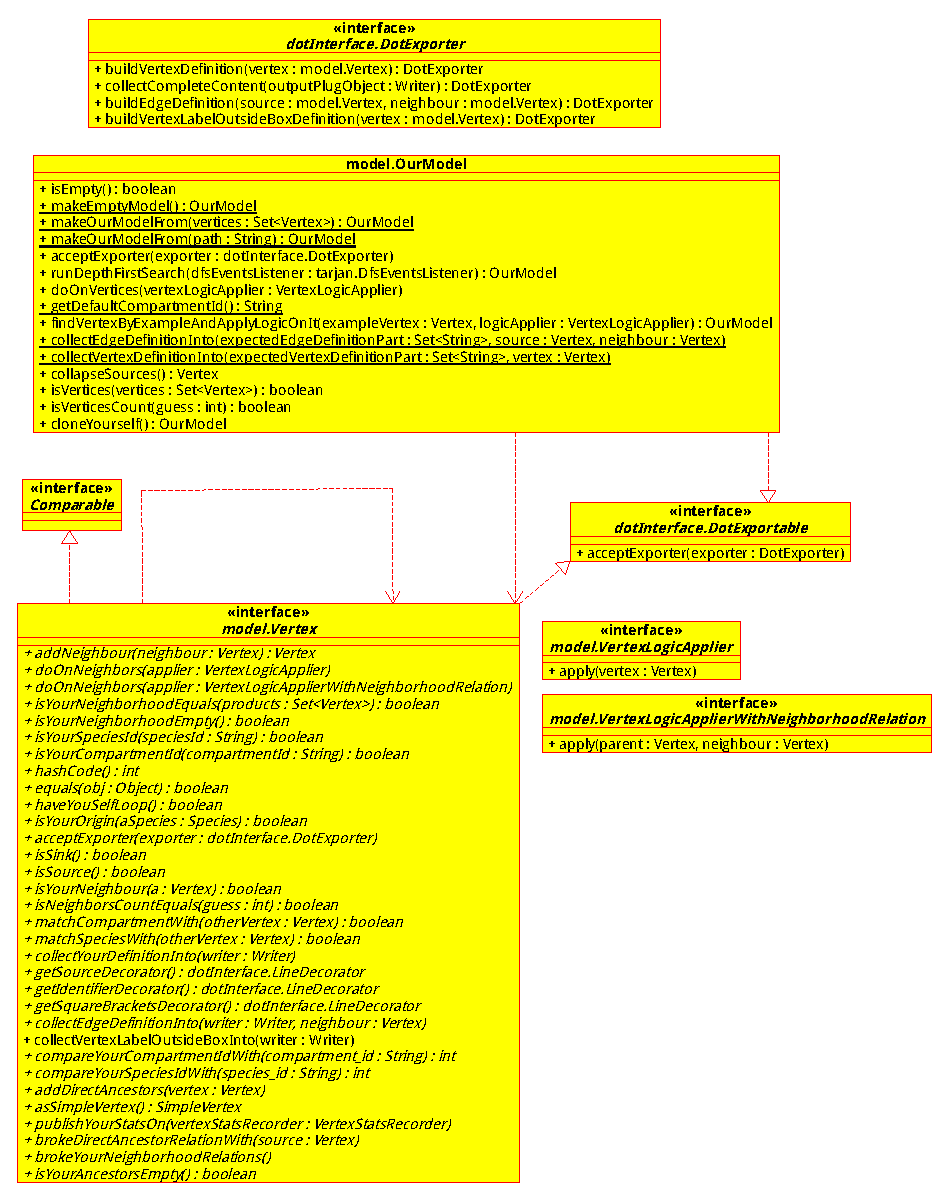
\includegraphics{packages/vertex-interface-class-diagram.eps} 
  \caption{Tarjan package's classes}
  \label{fig:tarjan-package-classes}
\end{figure}

\begin{paragraph}{DfsEventsListener}
Questo contratto permette di astrarre gli stati che si possono
incontrare durante una visita \emph{DFS} in modo da permettere non
solo l'implementazione della visita stessa, bensi anche di sue
varianti. Riporto sotto la sua definizione direttamente dal relativo
file sorgente:

\begin{lstlisting}
package tarjan; 
public interface DfsEventsListener {

  void searchCompleted(Map<Vertex, ExploreStatedWrapperVertex> map);
  void postVisit(Vertex v);
  void preVisit(Vertex v);
  void searchStarted(Map<Vertex, ExploreStatedWrapperVertex> map);
  void newVertexExplored(Vertex explorationCauseVertex, Vertex
    vertex);
  void fillCollectedVertices(Set<Vertex> vertices);
  void alreadyKnownVertex(Vertex vertex);
  }
\end{lstlisting}
Il motore che utilizza questa interfaccia \`e la classe
\emph{OurModel}. Aver definito questo contratto ci ha permesso di dare
una implementazione molto object-oriented, che differisce nello stile
rispetto ad una implementazione pi\`u comune in un linguaggio
procedurale. Credo sia interessante vederla, per cui mi dilungher\`o
in questi paragrafi nella sua descrizione. L'\emph{entry-point} della
computazione \`e il seguente metodo definito nella classe
\emph{OurModel}:
\begin{lstlisting}
  public OurModel runDepthFirstSearch(DfsEventsListener
  dfsEventsListener) { 
    final Map<Vertex, ExploreStatedWrapperVertex> map = makeDfsVertexMetadataMap();
    dfsEventsListener.searchStarted(map);
    for (Entry<Vertex, ExploreStatedWrapperVertex> entry : map.entrySet()) {
      entry.getValue().ifNotExplored(dfsEventsListener,	new
      ExploreStateWrapperVertexMapper() 
      {
        @Override
	public ExploreStatedWrapperVertex map(Vertex vertex) {
          return map.get(vertex);
	}
      });
    }
    dfsEventsListener.searchCompleted(map);
    return this;
  }
\end{lstlisting}
Questo metodo incapsula l'algoritmo della ricerca \emph{DFS}, usando
il listener passato come argomento, per notificare cosa st\`a
accadendo durante la ricerca. Come si nota, mancano alcuni pezzi per
avere una \emph{DFS} corretta: questi sono stati incapsulati nella
classe \emph{ExploreStateWrapperVertex} per avere un sistema pi\`u
object-oriented, rispetto a codificare tutto nel metodo sopra
riportato. La responsabilit\`a di questa nuova classe \`e quella di
associare ad ogni vertice l'informazione se questo \`e gia stato
visitato oppure no durante la visita. Inoltre, possiamo chiedere ad
oggetti istanze di questa classe, di esplorare il loro vicinato se non
sono gia stati esplorati, inviando il messaggio \emph{ifNotExplored}
che riporto:
\begin{lstlisting}
public class ExploredStateWrapperVertex...
  public ExploreStatedWrapperVertex ifNotExplored(
  final DfsEventsListener dfsEventsListener,
  Vertex explorationCauseVertex,
  final ExploreStateWrapperVertexMapper mapper) {
    final Vertex vertex = getWrappedVertex();
    if (isExplored() == false) {
      toggle();
      if (explorationCauseVertex != null) {
        dfsEventsListener.newVertexExplored(explorationCauseVertex,vertex);
      }
      dfsEventsListener.preVisit(vertex);
      vertex.doOnNeighbors(new VertexLogicApplierWithNeighborhoodRelation() {
        @Override
        public void apply(Vertex parent, Vertex neighbour) {
          if ((parent == vertex) == false) {
            throw new RuntimeException("Semantic error");
          }
          mapper.map(neighbour).ifNotExplored(dfsEventsListener,parent, mapper);
        }
      });
      dfsEventsListener.postVisit(vertex);
    } else {
      dfsEventsListener.alreadyKnownVertex(vertex);
    }
    return this;
}
\end{lstlisting}
Questo \`e il blocco mancante nel metodo precedente e che
effettivamente caratterizza la ricerca \emph{DFS} (linea 19). Nel
metodo sopra riportato inoltre si nota che \`e stato molto semplice
implementare questa parte, in quanto, data la natura ricorsiva
dell'implementazione, non dobbiamo far altro che invocare lo stesso
metodo su tutti i vertici del vicinato. Sar\`a il loro stato che
propagher\`a ancora il messaggio al rispettivo vicinato oppure, nel
caso il vertice sia gi\`a stato visitato, verr\`a segnalato al
listener questo evento inviando il messaggio
\emph{alreadyKnownVertex}. Una ultima osservazione deve essere fatta
riguardo agli eventi notificati: i listener concreti non per forza
devono definire della logica per ogni evento, in quanto ognuno di
questi viene creato per implementare una specifica variante e non
necessariamente ogni evento \`e richiesto per terminare quanto
desiderato.
\end{paragraph}

\begin{paragraph}{DfsEventsListenerTreeBuilder}
  Questo listener permette di associare ad ogni vertice delle
  informazioni per costruire l'albero \emph{DFS} che rappresenta la
  ricerca. In particolare si mantiene una coppia di istanti $(t_{in},
  t_{out})$ dove $t_{in}$ rappresenta l'istante in cui il vertice
  viene esplorato, $t_{out}$ rappresenta l'istante in cui si \`e
  finito di esplorare il rispettivo vicinato e la chiamata ricorsiva
  termina per tale vertice.

  Inoltre, nella gestione dell'evento \emph{newVertexExplored}, si
  costruisce la nuova relazione di vicinato, includendo solo quegli
  archi che hanno portato all'esporazione di nuovi vertici e che
  caratterizzano l'albero \emph{DFS} risultante.

  Riprendendo l'osservazione fatta al termine del paragrafo
  precedente, questo listener non ha bisogno di definire nessuna
  logica per l'evento \emph{alreadyKnownVertex}.
\end{paragraph}

\begin{paragraph}{TarjanEventsListenerTreeBuilder}
  Questo listener implementa l'algoritmo di Tarjan e codifica il
  comportamento per produrre un grafo i cui nodi sono le componenti
  fortemente connesse che si possono individuare nel grafo di
  input. 

  Questo grafo contiene come vertici degli oggetti che hanno
  comportamento specifico relativo alle componenti connesse, per cui,
  nelle successive computazioni, sar\`a possibile usare il grafo in
  modo astratto, inviando messaggi polimorfi che produrranno il
  comportamento desiderato (ad esempio la rappresentazione
  dell'etichetta nel documento grafico sar\`a diversa rispetto a
  quella che si pu\`o ottenere dopo una visita \emph{DFS}).
\end{paragraph}





% \section{Patterns and coding idioms}

\chapter{Conclusions}
\label{chapter:conclusions}


\section{TODO}
\begin{itemize}
\item dire che l'azione di compattare tutte le sorgenti \`e nata dal
  risultato della ricerca delle componenti fortemente connesse in
  quanto avevamo troppe sorgenti.
\end{itemize}

\section{Further work}

In questa sezione elenco alcuni punti che possono essere presi come
basi di partenza per sviluppi futuri del progetto. 

\begin{description}
\item[dependency injection] Rifattorizzare le parti del codice in cui
  vengono utilizzati degli oggetti \emph{factory} per nascondere la
  costruzione di realizzazioni specifiche di interfaccie (ad esempio
  come descritto in \nameref{itemize:model-supplied-abstraction}),
  sostituendole con motori di \emph{dependency injection}, applicando
  il principio di \emph{invertion of control}.
\item[domain specific language] speficare e implementare un \emph{DSL}
  per poter descrivere e assemblare la pipeline in modo dichiarativo,
  senza dover scendere al livello delle interfaccie e delle classi che
  abbiamo implementato. Questa dichiarazione potrebbe essere scritta o
  direttamente nella riga di comando oppure in un file esterno.
\item[graphviz interface] utilizzare una libreria che permette di
  usare programmaticamente gli oggetti e le implementazioni fornite
  dalla libreria \emph{graphviz}. Nell'attuale lavoro si utilizzano
  tali oggetti solo eseguendoli in modalit\`a di comando, equivalente
  ad una invocazione dal terminale \emph{bash}. Questo permetterebbe
  di avere un maggior grado di portabilit\`a del lavoro svolto,
  eliminando la dipendenza da una installazione a monte di
  \emph{graphviz}.
\item[configuration file] creare un file di configurazione nel quale
  si potrebbero impostare quale motore di \emph{graphviz} utilizzare
  per la renderizzazione dei grafi (ad esempio esistono anche
  \emph{neato} e molti altri) e il preambolo dei documenti dot nei
  quali si specifica le formattazioni, i colori di nodi e archi e le
  rispettive dimesioni.

  Inoltre potrebbe essere interessante esprire quanto detto nel
  precedente paragrafo con uno stesso DSL, in modo da poter esprire le
  proprie pipeline in batterie e lasciare al codice il codice di
  costruire i necessari oggetti ed eseguire le rispettive
  computazioni.
  % put here another further-work
\end{description}

\begin{thebibliography}{99}

\bibitem{SmalltalkCompanion98}
  Alpert, Brown, Woolf,
  \emph{The Design Pattern Smalltalk Companion}.
  Addison Wesley, Massachusetts,
  1st Edition,
  1998.

\end{thebibliography}

% \chapter{Internal organization}

% \section{Handwritten documents}

\subsection{Main plan}
\label{handwritten:MainPlan}
File: "/handwritten/20110830-MainPlan.jpg"

\subsection{Repo Structure}
\label{handwritten:RepoStructure}
File: "handwritten/20110902-RepoStructure.jpg"

% \section{On board journal}

\subsection{20110902}
Creato git repository e remote hosting on GitHub.com.
Aggiunto documento che cattura la sua struttura (vedi 
\ref{handwritten:RepoStructure}.

\subsection{20110830}
Incontro con prof. Crescenzi: progettato piano di lavoro. Vedi 
\ref{handwritten:MainPlan}.

\end{document} 

%%% Local Variables: 
%%% mode: latex
%%% TeX-master: t
%%% End: 
